%This template consists of the minimum of a single book.
%Please do not think this template is mandatory and the format must be followed strictly.
%We expect the author adds what he needs.
\documentclass[oneside,11pt,pdftex]{book}%Remove draft when book editing is completed.
\usepackage{graphicx}
\usepackage{amsmath}
%\usepackage{fontawesome5}
\usepackage{booktabs}
\usepackage{amssymb}	
\usepackage{longtable}
\usepackage{amsthm}
\usepackage{multirow}
\usepackage[activate={true,nocompatibility},final,tracking=true,kerning=true,spacing=true,factor=1100,stretch=10,shrink=10]{microtype}
\usepackage[toc,page]{appendix}
\usepackage[nottoc]{tocbibind}
\numberwithin{equation}{section}
\graphicspath{ {./Images/} }
%\usepackage[raggedright]{titlesec}
\usepackage{placeins}
\usepackage{mathtools}


\usepackage{fancyhdr}
\usepackage{hyperref}
%Be careful when you use commands which align formulas.
%If aligned formulas range to two pages, the formulas should be divided into two environments.
%\makeatletter
%\AtBeginDocument{\let\mathaccentV\AMS@mathaccentV}
%\makeatother
%This is a patch for double bar.
%Activate it if \bar{\bar{a}} doesn't work.

\newskip\thskip
\thskip=0.5\baselineskip plus 0.2\baselineskip minus 0.2\baselineskip

\newdimen\dtest%Remove this when book editing is completed.
\settowidth{\dtest}{letters and symbols here}
\typeout{<<<\the\dtest>>>}

\newtheorem{theorem}{Theorem}[chapter]%Modify these declarations for your need.
\newtheorem{lemma}[theorem]{Lemma}
\newtheorem{corollary}[theorem]{Corollary}
\newtheorem{example}[theorem]{Example}
\newtheorem{definition}[theorem]{Definition}

\newtheorem{xca}[theorem]{Exercise}

\newtheorem{remark}[theorem]{Remark}

\numberwithin{section}{chapter}
\numberwithin{equation}{chapter}

\makeindex

\newcommand{\R}{\mathbb{R}}
\newcommand{\Q}{\mathbb{Q}}
\newcommand{\C}{\mathbb{C}}
\newcommand{\Z}{\mathbb{Z}}
\newcommand{\N}{\mathbb{N}}
\newcommand{\D}{\mathbb{D}}
\newcommand{\F}{\mathbb{F}}

\graphicspath{ {graphics/} }
\newcommand\numberthis{\addtocounter{equation}{1}\tag{\theequation}}
\begin{document}


\frontmatter

\thispagestyle{empty}
\begin{flushright}
{\LARGE \textbf{Bhoris Dhanjal}}%Input your name here.
\end{flushright}
\vfill
\begin{center}
{\fontsize{29.86truept}{0truept}\selectfont \textbf{Probability and Sampling Distributions (B)}}%Input the book title here.
%Below is for a book with a subtitle.
%{\fontsize{29.86truept}{0truept}\selectfont \textbf{The Book Title}} \\
%\vspace{6.5truept}
%{\Large, \LARGE, etc. \textbf{The Subtitle}}
\end{center}
\vfill
\begin{flushleft}
{\LARGE \textbf{Lecture Notes}} \\
\hspace{-1.75truept}
{\large \textbf{for SSTA401}}
\end{flushleft}
\newpage

\tableofcontents


\mainmatter

\chapter[Continuous probability distributions]{Transformation of random variables \& standard univariate continuous probability distributions}
\section{Uniform/Rectangular distributions}
\begin{definition}\label{def:uniformdist}
	A r.v. $ X$ is said to follow uniform distribution over an interval $ (a,b) $ if its pdf is constant over the entire range.
\end{definition}
\subsection{PDF of uniform distribution}
\begin{theorem}
	PDF of uniform distribution
	\begin{align*}
		P(x)&=k && a<x<b\\
		&=0 && \text{otherwise}
	\end{align*}
\end{theorem}



\begin{itemize}
	\item $ \int_a^b f(x)\, dx=\int_a^b k\, dx = k[x]_a^b=k(b-a)=1$, therefore $k= \frac{1}{b-a} $
	\item We denote it as, $ X \sim U(a,b) $
	\item $ f(x)=\frac{1}{b-a} $\\ 
\end{itemize}

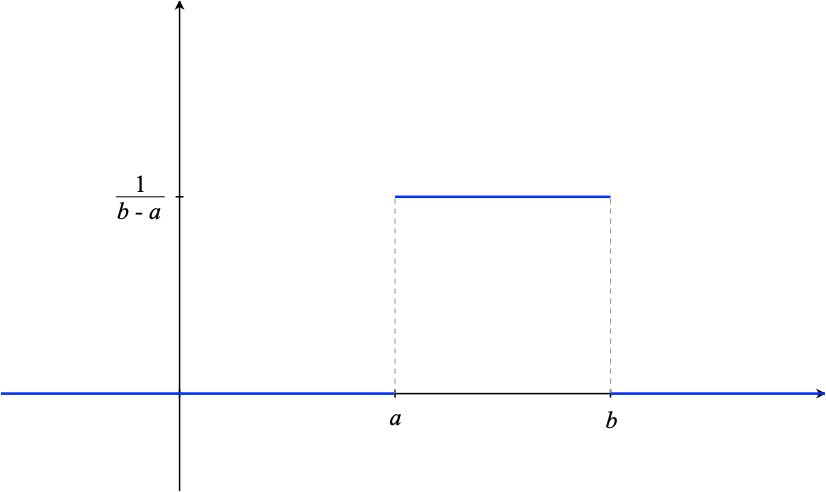
\includegraphics[scale=0.3]{uniform}

\subsection{CDF of uniform distribution}
\begin{theorem}\label{ref:cdfuniform}
	CDF of uniform distribution
	\begin{align*}
		F(x)&=0 && x \leq a\\
		&= P(X\leq x)= \int_a^x f(x)\,dx=\frac{x-a}{b-a} && a<x<b\\
			&=1 && x\geq b
	\end{align*}
\end{theorem}


\subsection{Expectation and variance of uniform distribution}
\begin{theorem}
	Expected value of $ X \sim U(a,b) $ is equal to $\frac{(a+b)}{2}$
\end{theorem}


\begin{proof}
	Consider the expectation of the uniform distribution as,
	\begin{align*}
		E[x]&=\int_a^b x P(x)\, dx\\
		&= \int_a^b x \frac{1}{b-a}\, dx\\
		&= \frac{1}{b-a} \int_a^b x\, dx\\
		&= \frac{a+b}{2}
	\end{align*}
\end{proof}

\begin{theorem}
	Variance of uniform distribution is equal to $ \frac{1}{12} (b-a)^2$
\end{theorem}
\begin{proof}
	We begin by finding out $ E[X^2] $
	\begin{align*}
		E[X^2]&=\int_a^b x^2 P(x)\, dx\\
		&= \int_a^b x^2 \frac{1}{b-a}\, dx\\
		&= \frac{1}{b-a}\int_a^b x^2\, dx\\
		&= \frac{1}{3}\left( a^2+ab+b^2\right)
\intertext{Now we can find the variance as $ V[X]=E[X^2]-E[X]^2 $ as follows,}
		V[X]&=E[X^2]-E[X]^2\\
		&= \frac{1}{3}\left( a^2+ab+b^2\right)-\left( \frac{a+b}{2}\right)^2\\
		&=\frac{(b-a)^2}{12}
	\end{align*}
\end{proof}


\subsection{Raw moments of uniform distribution}
The $ r^{th} $ raw moment of the uniform distribution is given as 

\begin{align*}
	\mu_r'&=E[X^r]=\int_a^b x^r f(x)\, dx \\
	&= \frac{1}{b-a}\left[ \frac{x^{r+1}}{r+1} \right]_a^b=\frac{b^{r+1}-a^{r+1}}{(b-a)(r+1)}
\end{align*}


\begin{example}
	Suppose in a quiz there are 30 participants. A question is given to all 30 participants and the time allowed is 25 seconds. 
\end{example}
\begin{proof}
	Let $ X$ denote the time to respond.\\
	$ X \sim U(0,25) $, the pdf is given by 
	$ f(x) =\frac{1}{25}; 0<x<25$ and $ 0 $ otherwise.
	$$ P(x\leq 6)=\int_0^6 f(x)\, dx=\int_0^6 \frac{1}{25}\, dx = \frac{151}{25}$$
	\[P(6 \leq x \leq 10)=\int_6^10 f(x)\, dx = \int_6^{10} \frac{1}{25}\, dx= \frac{101}{25} \]
\end{proof}

\begin{example}
	A r.v. $ x $ is said to follow uniform dist with $ \mu=1 $ and $ V(x) = 4/3$. Obtain $ P(x<0) $.
\end{example}
\begin{proof}
	First begin by finding out the parameters for the unfirom distribution.\\
	First consider the mean,
	\begin{align*}
		\mu&=1\\
		\frac{a+b}{2}&=1\\
		a+b&=2
	\end{align*}
	Then consider the variance,
	\begin{align*}
		V(x)&=\frac{4}{3}\\
		\frac{(b-a)^2}{12}&=\frac{4}{3}\\
		(b-a)^2&=16
	\end{align*}
	Solving two simultaneous equations we get $ a=-1, b=3 $.\\
	Therefore, we have $ X \sim U(-1,3) $\\
	\begin{align*}
		P(x\leq0)&=F(0)=\frac{0+1}{4}=\frac{1}{4}
	\end{align*}
\end{proof}


\begin{example}
	If $ X \sim U(-3,3) $, find $ P(x<2) $, $ P(|x|<2) $, $ P(|x-2|<2),$ also obtain $ k $ if $ P(x>k) =1/3$
\end{example}
\begin{proof}
	\begin{align*}
		P(x<2)&=F(2)=\frac{2+3}{6}=
		\frac{5}{6}\\
		P(|x|<2)&=\int_-2^2 \frac{1}{6}\, dx = \frac{2}{3}\\
		P(|x-2|<2)&=\int_0^3 \frac{1}{6}=\frac{1}{2}\\
		P(x>k)=1/3\implies \dots
	\end{align*}
	Complete this l8r alig8r
	
\end{proof}

\subsection{MGF of Uniform distribution}
\begin{theorem}
	MGF of Uniform distribution  $= \frac{e^{bt}-e^{at}}{t(b-a)}, t\neq0 $ and $ =1, t=0 $
\end{theorem}
\begin{proof}
	\begin{align*}
		M_x(t)&=E[e^{tx}]=\int_a^b \frac{e^{tx}}{b-a}\, dt= \frac{e^{bt}-e^{at}}{(b-a)t}
		\intertext{The Taylor series for this can be expressed as the following,}
		M_x(t)&=\frac{b-a}{b-a}+\frac{b^2-a^2}{2(b-a)}t+\frac{b^3-a^3}{3(b-a)}\frac{t^2}{2!}+\cdots
	\end{align*}
	Therefore we can say, 
	\begin{align*}
		 \mu_1'&= \text{coeff of } t=\frac{b^2-a^2}{2(b-a)}=\frac{a+b}{2}\\
		 \mu_2'&= \text{coeff of }\frac{t^2}{2!}=\frac{b^3-a^3}{3(b-a)}
	\end{align*}
And we can say $ \mu_2 = \dots$ 
\end{proof}

\subsection{Applications of uniform distribution}
\begin{enumerate}
	\item Assumption of uniform death for insurance\\
    $ \vdots $
\end{enumerate}
Write sumthin here

\section{Gamma distribution}
\begin{definition}[Gamma distribution]
	A r.v. $ `X' $ is said to follow gamma distribution $ X \sim G(\lambda, \theta) $. Where $ \lambda=$ shape parameter and $ \theta= $ scale parameter.
\end{definition}

\subsection{PDF of Gamma distribution}
\begin{definition}[PDF of Gamma distribution]
	\begin{align*}
		f(x,\lambda, \theta)&=\frac{\theta^{\lambda}}{\Gamma (\lambda)} e^{-\theta x} x^{\lambda -1}&& x>0, \lambda>0, \theta>0\\
		&= 0 && \text{otherwise}
	\end{align*}
Where $ \Gamma (\lambda)=(\lambda-1)!=(\lambda-1)\Gamma (\lambda -1) $.\\
\end{definition}





\begin{corollary}
	If $ \theta=1 $ we will have gamma distribution with a single parameter $ \lambda $ which is called the standard gamma distribution.
	\begin{align*}
		X\sim G(\lambda)&= \frac{e^{-x} x^{\lambda -1}}{\Gamma (\lambda )} && x>0, \lambda >0\\
		&=0 && \text{otherwise}
	\end{align*}
\end{corollary}

\begin{corollary}
	If $ \lambda=1, X \sim G(1, \theta) = \text{Exp}(\theta)$.
\end{corollary}

\begin{corollary}
	If $ \lambda=1, \theta=1 $, $ X \sim  $ Standard exponential distribution, i.e.
	\begin{align*}
		f(x)&= e^{-x} && x>0\\
		&=0 && \text{otherwise}
	\end{align*}
\end{corollary}


\begin{definition}[Gamma function]
	\[ \Gamma(\lambda) =\int_0^\infty e^{-x} x^{\lambda -1 }\, dx \]
\end{definition}

\begin{definition}[Gamma integral]
	\[ \int_0^\infty e^{- \theta x} x^{\lambda -1}\, dx = \frac{\Gamma (\lambda)}{\theta^\lambda}\]
\end{definition}

\subsection{CDF of Gamma distribution}
\begin{theorem}
 	CDF of Gamma distribution is given as \[ F(x) = \]
\end{theorem}
\begin{proof}
	\begin{align*}
		F(x)&=P(X<x)=\int_0^x \frac{\theta ^\lambda e^{- \theta x} x^{\lambda -1}}{\Gamma (\lambda )}\, dx\\
		&=\frac{\theta^{\lambda}}{\Gamma(\lambda)} \int_0^x x^{\lambda-1} e^{-\theta x}\, dx
	\end{align*}
\end{proof}

\subsection{Raw moments of Gamma distribution}
\begin{theorem}
	The $ r^{th} $ raw moment of the Gamma distribution is given by \[\mu_r'=\frac{\Gamma(\lambda+r)}{\Gamma(\lambda)\theta^r} \]
\end{theorem}
\begin{proof}
	\begin{align*}
		\mu_r'=E[x^r]&=\int_0^\infty \frac{x^r \theta^\lambda e^{-\theta x} x^{\lambda -1}}{\Gamma(\lambda)}\, dx\\
		&=\int_0^{\infty} \dfrac{\theta^{\lambda} e^{-\theta x}x^{\lambda+r-1}  }{\Gamma(\lambda)}\, dx\\
		&= \frac{\Gamma(\lambda+r)}{\Gamma(\lambda) \theta^r}
	\end{align*}
\end{proof}

\subsection{Mean and Variance of Gamma distribution}
Now we can find $ \mu_1', \mu_2' $
\begin{align*}
	E[x]= \mu_1'&=\frac{\lambda}{\theta}\\
	\mu_2'&= \frac{\lambda(\lambda+1)}{\theta^2}\\
	V[x] = \mu_2 &=\mu_2'-\mu_1'^2=\frac{\lambda(\lambda +1)}{\theta^2}-\frac{\lambda^2}{\theta^2}=\frac{\lambda}{\theta^2}
\end{align*}

\subsection{MGF of Gamma distribution}
\begin{align*}
	 E[e^{tx}]&=\int_0^{\infty} e^{tx} \frac{\theta^\lambda e^{-\theta x} x^{\lambda -1}}{\Gamma(\lambda )}\, dx\\
	 &= \frac{\theta^{\lambda}}{\Gamma (\lambda)} \int_0^{\infty} e^{-(\theta - t) x}x^{\lambda -1}\, dx\\
	 &= \frac{\theta^\lambda}{\Gamma(\lambda )} \frac{\Gamma(\lambda )}{(\theta -t )^{\lambda}}=\left( \frac{\theta}{\theta - t}\right)^\lambda\\
	 &=\left(1- \frac{t}{\theta}\right)^{- \lambda}
\end{align*}

\subsection{CGF of Gamma distribution}
\begin{align*}
	K_x(t)&=\log \left( 1- \frac{t}{\theta} \right)^{-\lambda}\\
	&= -\lambda \log \left(1- \frac{t}{\theta}\right)\\
	&= \frac{\lambda t }{\theta }+\frac{\lambda t^2}{2 \theta^2}+\frac{\lambda t^3}{3 \theta^3}+ \cdots
\end{align*}
Using this we can get the mean and variance easily.
\begin{align*}
	\text{Mean }&=k_1=\frac{\lambda }{\theta}\\
	\text{Variance }&= k_2= \frac{\lambda }{\theta^2}
	\end{align*}

\subsection{Additive property of Gamma distribution}
If $ X_i (i=1,\dots, k) $ are $ k $ independent Gamma distributions with parameters $ \lambda_1, \lambda_2, \dots, \lambda_k  $ and $ \theta  $ respectively, then,
\begin{align*}
	\sum_{i=1}^{k}X_i &\sim G \left( \sum_{i=1}^{k} \lambda_i, \theta \right)\\
	M_{X_i}(t)&= \left(1 -\frac{t}{\theta} \right)^{-\lambda_i}
	\intertext{Let $ Z=\sum X_i $}
	M_Z(t)&= \prod_{i=1}^k \left(1- \frac{t}{\theta}\right)^{-\lambda_i}\\
	&= \left(1- \frac{t}{\theta}\right)^{- \sum \lambda_i}
	\intertext{By uniqueness property of mgf}
	\sum_i X_i &\sim G \left(\sum_i \lambda_i, \theta \right)
\end{align*}

\subsection{Limiting form of Gamma distribution}
\begin{align*}
	\beta_1 &= \frac{4}{\lambda}, \text{ as $ \lambda \rightarrow \infty $}, \beta_1 \rightarrow 0 \implies \text{Normal dist}\\
	\beta_2 &= 3+ \frac{6}{\lambda } \text{ as $ \lambda \rightarrow \infty $}, \beta_2 \rightarrow 3 \implies \text{Normal dist}
\end{align*}
Note that they are both independent of $ \theta  $.\\
Therefore, as $ \lambda \rightarrow \infty  $ we have $ G(\lambda , \infty ) \rightarrow N \left(\frac{\lambda}{\theta}, \frac{\lambda }{\theta^2}\right)$.

\subsection{Applications of Gamma distribution}
Idk write something bruh

\section{Exponential distribution}
\subsection{PDF of Exponential Distribution}
\begin{definition}[PDF of Exponential distribution]
	A r.v. $ x $ is said to follow the exponential distribution with parameter $ \theta  $ if its pdf is given by 
	\begin{align*}
		f(x)&= \theta e^{-\theta x} && x\geq 0, \theta > 0\\
		&= 0 && \text{otherwise}
	\end{align*}
\end{definition}


\subsection{INCOMPLETE CDF of exponential distribution}
\begin{align*}
	F[x]=1-e^{-\theta x}
\end{align*}
\textbf{FILL THIS UP}
\subsection{Raw moment of exponential distribution}

\begin{theorem}
	The $ r^{th} $ raw moment for exponential distribution is given by \[ \mu_r'=\frac{r!}{\theta^r} \]
\end{theorem}
\begin{proof}
	\begin{align*}
		\mu_r'=E[x^r]&=\int_0^\infty x^r \theta e^{-\theta x}\, dx\\
		&=\frac{\Gamma(r+1)}{\theta^r}\\
		&= \frac{r!}{\theta^r}
	\end{align*}
\end{proof}

\subsection{Mean and variance of exponential distribution}
\begin{theorem}
	The mean of exponential distribution is given be \[ \mu=\frac{1}{\theta} \]
\end{theorem}
\begin{proof}
	Consider $ r=1 $,
	\begin{align*}
		\mu_1'=\frac{1}{\theta}
	\end{align*}
\end{proof}

\begin{theorem}
	The variance of the exponential distribution is given by \[ \mu_2 = \frac{1}{\theta^2}\]
\end{theorem}
\begin{proof}
	First find $ \mu_2' $
	\begin{align*}
		\mu_2'=\frac{2}{\theta^2}
	\end{align*}
So now we can compute the variance as $ \frac{1}{\theta^2} $
\end{proof}

\subsection{MGF of exponential distribution}
\begin{theorem}
	MGF of exponential distribution is given by \[ M_x(t)= \left(1- \frac{t}{\theta}\right)^{-1} \]
\end{theorem}
\begin{proof}
	\begin{align*}
		M_x(t)&=E[e^{tx}]\\
		&=\int_0^\infty e^{tx} \theta e^{-\theta x}\, dx\\
		&=\theta \int_0^\infty e^{x(t-\theta)} x^{1-1}\, dx\\
		&= \frac{\theta \Gamma(1)}{\theta - t}\\
		&=\frac{\theta }{\theta-t}\\
		&= \left(1- \frac{t}{\theta}\right)^{-1}
	\end{align*}
\end{proof}

\subsection{CGF of exponential distribution}
\begin{theorem}
	CGF of exponential distribution is given by \[ K_x(t)=-\log\left(1- \frac{t}{\theta}\right) \]
\end{theorem}
\begin{proof}
	\begin{align*}
		K_x(t)&= \log \left(1-\frac{t}{\theta}\right)^{-1}\\
		&= -\log\left(1- \frac{t}{\theta}\right)\\
		&= \frac{t}{\theta }+\frac{t^2}{2 \theta^2}+\frac{t^3}{3 \theta^3}
	\end{align*}
We can say the general $ r^{th} $ cumulant is given by $ K_r=\frac{(r-1)!}{\theta^r} $
\end{proof}

\subsection{Additive property of exponential variates}
\begin{theorem}
	If $ x_1,x_2,\dots,x_k $ are $ k $ independent exponential variates each with parameter $ \theta  $then \[ \sum_{i=1}^k x_i \sim G(k, \theta)\]
\end{theorem}
\begin{proof}
	We will do this with the MGF. Consider taht $ Z=\sum{i=1}^{k} x_i $.
	\begin{align*}
		M_z(t)&=\prod_{i=1}^{k} M_x(t)\\
		&= \prod_{i=1}^k \left(1- \frac{t}{\theta}\right)^{-1}\\
		&= \left(1- \frac{t}{\theta}\right)^{-k}
	\end{align*}
Therefore, (by uniqueness property of MGF) comparing this MGF to that of the gamma distribution we can say that,
$$ \sum_{i=1}^k x_i = Z \sim G(k,\theta)$$
\end{proof}

\subsection{Lack of memory of exponential distribution}
\begin{theorem}
	For a exponentially distributed random variate, $ P[x>a+b \mid x>a]=P[x>b] $
\end{theorem}
\begin{proof}
	Let $ X \sim E(\theta) $. Consider first case
	\begin{align*}
		P[x>a+b \mid x>a]&= \frac{P[x>a+b]}{P[x>a]}\\
		&=\frac{\int_{a+b}^\infty \theta e^{-\theta x}\, dx}{\int_a^\infty \theta e^{-\theta x}\, dx}\\
		&=\frac{e^{-\theta a+b}}{e^{-\theta a}}\\
		&=e^{-\theta b}
	\end{align*}
	Consider second case now,
	\begin{align*}
		P[x>b]&=\int_b^{\infty }\theta e^{-\theta x}\, dx=e^{-\theta b}
	\end{align*}
	Equality holds.
\end{proof}

\section{INCOMPLETE Laplace distribution (Double exponential)}
\subsection{PDF}
\begin{definition}[PDF of Laplace distribution]
	$ X\sim L (\lambda, \mu)$\[ f(x)=\begin{cases}
		\frac{1}{2 \lambda } e^{-\left|\frac{x-\mu }{\lambda}\right|} & -\infty<x<\infty\\
		0 & \text{otherwise}
	\end{cases} \]
\end{definition}
\subsection{CDF}
\begin{definition}[CDF of Laplace distribution]
	\[ F[x]=\begin{cases}
		content...
	\end{cases} \]
\end{definition}

\subsection{Raw moment}
\begin{theorem}
	The $ r^{th} $ raw moment for the Laplace distribution is given by \[ \mu_r'= \]
\end{theorem}
\begin{proof}
	\begin{align*}
		\mu_r'&=E[x^r]=\int_{-\infty}^\infty \frac{x^r}{2 \lambda }e^{-\left|\frac{x-\mu }{\lambda}\, dx\right|}
		\intertext{Transform $ (x-\mu)/\lambda =z $}
		&=\frac{1}{2\lambda }\left( \int_{-\infty}^\infty (z\lambda+\mu)^r e^{-|z|}\, \lambda\, dz  \right)\\
		&=\frac{1}{2} \left(\int_{-\infty}^\infty \sum_{k=0}^{r}\binom{r}{k} (z-\lambda)^k \mu^{r-k} e^{-|z| \, dz}\right)\\
		&=\frac{1}{2}\sum_{k=0}^r \left[\binom{r}{k}\lambda^k \mu^{r-k} \int_{-\infty}^\infty z^k e^{-|z|}\, dz \right]\\
		\intertext{Complete this up}
		&=\frac{1}{2}\sum_{k=0}^{r} \left[\binom{r}{k} \lambda^k \mu^{r-k} k! (1+(-1)^k)\right]
	\end{align*}
\end{proof}

\subsection{Mean and variance}
We can do this with the raw moments above but instead we will do it with the PDF.
\begin{theorem}
	Expectation of laplace distribution is given as \[ E[x]= \]
\end{theorem}
\begin{proof}
	\begin{align*}
		E[x]&=\int_{-\infty }^{\infty }x f(x)\, dx\\
		&=\int_{-\infty }^{\infty }\frac{x}{2\lambda}e^{-\left|\frac{x-\mu }{\lambda}\right|}\, dx
		\intertext{Split it around $ \mu $}
		&=\frac{1}{2\lambda}\left( \int_{-\infty}^\mu x e^{\frac{x-\mu }{\lambda}}\, dx + \int_\mu^{\infty}x e^{-\frac{x-\mu }{\lambda}}\, dx \right)\\
		&= \frac{1}{2\lambda} \left[ e^{-\mu/ \lambda}\int_{-\infty}^{\mu} xe^{x/\lambda}\, dx + e^{\mu/\lambda}\int_{\mu}^{\infty}xe^{-x/\lambda}\, dz\right]\\
		&=\frac{1}{2 \lambda} \left[e^{-\mu/\lambda } \lambda(x-\lambda)e^{x/ \lambda}-e^{\mu/\lambda }(\lambda(x+\lambda)e^{-x/ \lambda}) \right]\\
		&=\mu
	\end{align*}
\end{proof}

\begin{theorem}
	Expectation of $ x^2 $ in Laplace distribution is given be \[ E[x^2]=bruh \]
\end{theorem}
\begin{proof}
	\begin{align*}
		E[x^2]&=\int_{-\infty}^\infty x^2 \frac{1}{2\lambda }e^{-\left| \frac{x-\mu }{\lambda} \right|}
		\intertext{Split it around $ \mu $}
		&=\frac{1}{2\lambda}\left( \int_{-\infty}^\mu x^2 e^{\frac{x-\mu }{\lambda}}\, dx + \int_\mu^{\infty}x^2 e^{-\frac{x-\mu }{\lambda}}\, dx \right)\\
		&= \frac{1}{2\lambda} \left[ e^{-\mu/ \lambda}\int_{-\infty}^{\mu} x^2e^{x/\lambda}\, dx + e^{\mu/\lambda}\int_{\mu}^{\infty}x^2e^{-x/\lambda}\, dx\right]\\
		&= \frac{1}{2\lambda} \left[ e^{-\mu/ \lambda}(\lambda (x^2-2\lambda x+2\lambda^2)e^{x/\lambda}) - e^{\mu/\lambda}(\lambda(x^2+2\lambda x+2\lambda^2)e^{-x/ \lambda})\right]\\
		&=2\lambda^2
	\end{align*}
\end{proof}
\begin{theorem}
	Variance of Laplace distribution is given as \[ V[x]= \]
\end{theorem}


\subsection{MGF}
\begin{theorem}
	MGF of the Laplace distribution is given by \[ M_x(t)=bruh \]
\end{theorem}
\begin{proof}
	\begin{align*}
		M_x(t)&=E[e^{tx}]=\int_{-\infty}^\infty \frac{1}{2\lambda} e^{tx-\left|\frac{x-\mu }{\lambda}\right|}\\
		&=\frac{1}{2\lambda}\left[e^{-\mu/\lambda} \int_{-\infty}^\mu e^{x\left(t+\frac{1}{\lambda} \right)}\, dx + e^{\mu/\lambda}\int_\mu^{\infty} e^{-x\left(\frac{1}{\lambda}-t \right)}\, dx\right]\\
		&= \frac{1}{2 \lambda } \left[e^{-\mu/\lambda} \left(\frac{e^{\mu \left( \frac{1}{\lambda} +t \right)}}{\frac{1}{\lambda}+t}\right) + e^{\mu/\lambda} \left(\frac{-e^{\mu \left(\frac{1}{\lambda}-t \right)}}{-\frac{1}{\lambda} +t}\right)\right]\\
		&=\frac{1}{2\lambda }\left[\frac{e^{\mu t}}{t+\frac{1}{\lambda}}-\frac{e^{\mu t}}{t-\frac{1}{\lambda}}\right]
	\end{align*}
\end{proof}

Plot a graph for the beta-1 dsitribution when alpha=5, beta=2
\subsection{CGF}

\section{Beta distribution of Type-I}
\subsection{PDF}
\begin{definition}[PDF of Beta I]
	\[ f(x)=\begin{cases}
		\frac{1}{\beta(m,n)}x^{m-1}(1-x)^{n-1} & 0<x<1; m,n>0\\
		0 & \text{otherwise}
	\end{cases} \]
	Where $ \beta(m,n) = \frac{\Gamma(m)\Gamma(n)}{\Gamma(m+n)}$
\end{definition}
Note the following,
\begin{enumerate}
	\item We can say, $ X \sim \beta_1 (m,n) $ where $ m,n $ are the parameters of the distribution.
	\item Since $ f(x) $ is a pdf we have the following,
	\begin{align*}
		\int_0^1 f(x)\, dx &= \int_0^1 \frac{1}{\beta(m,n)} x^{m-1} (1-x)^{n-1}\, dx\\
		&= \int_0^1 
	\end{align*}
\end{enumerate}

\subsection{Raw moments}
\begin{theorem}
	The $ r^{th}$ raw moment of the Beta I distribution is given by \[ \mu_r'=\frac{\Gamma(m+n)\Gamma(r+m)}{\Gamma(m)\Gamma(m+n+r)} \]
\end{theorem}
\begin{proof}
	\begin{align*}
		\mu_{r}'=E[x^r]&=\int_0^1 \frac{1}{\beta(m,n)} x^{r+m-1}(1-x)^{n-1}\, dx\\
		&=\frac{\Gamma(m+n)\Gamma(r+m)}{\Gamma(m)\Gamma(m+n+r)}
	\end{align*}
\end{proof}

\subsection{Mean and Variance}
\begin{theorem}
	Mean of Beta I distribution is given by \[ E[x]=\frac{m}{m+n} \]
\end{theorem}
\begin{proof}
	\begin{align*}
		E[x]=\mu_1'=\frac{\Gamma(m+n)\Gamma(m+1)}{\Gamma(m)+\Gamma(m+n+1)}=\frac{m}{m+n}
	\end{align*}
\end{proof}

\begin{theorem}
	Variance of Beta I distribution is given by \[ V[x]=\frac{mn}{(m+n)^2(m+n+1)} \]
\end{theorem}
\begin{proof}
	\begin{align*}
		\mu_2'&=\frac{(m+1)(m)}{(m+n)(m+n+1)}
	\end{align*}
So now we have the variance given as,
\begin{align*}
	\mu_2&=\mu_2'-\mu_1'^2\\
	&=\frac{mn}{(m+n)^2(m+n+1)}
\end{align*}
\end{proof}

\section{Beta distribution of Type-II}
\subsection{PDF}
\begin{definition}[PDF of Beta-II distribution]
	\[ f(x)=\begin{cases}
		\frac{1}{\beta(m,n)}\frac{x^{m-1}}{(1+x)^{m+n}} & 0<x<\infty; m,n>0\\
		0 & \text{otherwise}
	\end{cases} \]
\end{definition}
Note the following,
\begin{enumerate}
	\item $ X $ is said to follow $ \beta_2(m,n) $ as $ X \sim \beta_2(m,n) $
	\item \begin{align*}
		\int_0^{\infty }f(x)\, dx&=\int_0^\infty \frac{x^{m+1}}{(1+x)^{m+n}}=\beta(m,n)
	\end{align*}
\end{enumerate}

\subsection{Raw moments}
\begin{theorem}[Raw moments of Beta-2 distribution]
	The raw moments of the Beta-2 distribution is given by \[ \mu_r'= \frac{\Gamma(m+r)\Gamma(n-r)}{\Gamma(m)\Gamma(n)} \]
\end{theorem}
\begin{proof}
	\begin{align*}
		\mu_r'&=E[x^r]=\int_0^{\infty} \frac{1}{\beta(m,n)}\frac{x^{m+r-1}}{(1+x)^{m+n}}\, dx\\
		&=\frac{\Gamma(m+r)\Gamma(n-r)}{\Gamma(m)\Gamma(n)}
	\end{align*}
\end{proof}

\subsection{Mean and variance}
\begin{theorem}[Mean of Beta-2 distribution]
	The mean of Beta-2 distribution is given by \[ E[x]=\frac{m}{n-1} \]
\end{theorem}
\begin{proof}
	\begin{align*}
		E[x]&=\mu_1'=\frac{\Gamma(m+1)\Gamma(n-1)}{\Gamma(m)\Gamma(n)}\\
		&=\frac{m}{n-1}
	\end{align*}
\end{proof}

\begin{theorem}[Variance of Beta-2 distribution]
	The variance of Beta-2 distribution is given by \[ V[x]=\frac{m(m+n-1)}{(n-2)(n-1)^2} \]
\end{theorem}
\begin{proof}
	First consider the 2nd raw moment,
	\begin{align*}
		\mu_2'&=\frac{m(m+1)}{(n-2)(n-2)}
	\end{align*}
	Now we can compute the variance as follows
	\begin{align*}
		V[x]&=\mu_2=\mu_2'-\mu_1'^2=\frac{m(m+n-1)}{(n-2)(n-1)^2}
	\end{align*}
\end{proof}

\section{Transformation of variables}
\subsection{One dimensional random variable}
Let $ X $ be a continuous random variable with pdf $ f(x) $ and let $ Y=g(x) $ be a strictly monotonic function of $ X $ with unique inverse.\\
Assume that $ g(x) $ is differentiable and is continuous for all $ x $, then the pdf of r.v. $ Y $ is given by 
\[ h(y)=f(x) \cdot \det \left|\frac{dx}{dy}\right| = \left|\frac{dx}{dy}\right|\]
where r.v. $ x $ is expressed in terms of $ y $.
Steps to solve,
\begin{enumerate}
	\item Write pdf of r.v. $ X $.
	\item Express old variable $ X $ in terms of new variable $ Y $.
	\item Write the range of the new variable.
	\item Obtain $ J $ where $ J=\left|\frac{dx}{dy}\right| $ and $ |J| $.
	\item Obtain $ h(y) =f(x)\cdot |J|,$ where $ X $ is expressed in terms of $ Y. $
\end{enumerate}
\begin{remark}
		For $ 2-1 $ correspondence, i.e. for ever 2 values of $ X $ is there is only one value of $ Y $, then multiple $ |J| $ with 2.
\end{remark}
\begin{remark}
	\item For $ 1-2 $ correspondence i.e., for every 1 value of x if there are 2 values of $ Y $ then multiply $|J| $ with $ \frac{1}{2} $.
\end{remark}

\begin{example}
	If a r.v. $ X \sim B_1(m,n) $ obtain the distribution of $ Y=1-X $.
\end{example}
\begin{proof}
	First begin by stating the pdf of $ X $.
	\begin{align*}
		f(x)=\begin{cases}
			\frac{1}{\beta(m,n)}x^{m-1}(1-x)^{n-1} & 0<x<1; m,n>0\\
			0 & \text{otherwise}
		\end{cases} 
	\end{align*}
	Now $ X=1-Y $ this ranges from $ 1-Y=0 $ to $ 1-Y=1 $. So $ 0<Y<1 $ again.\\
	Now compute $ J $
	\begin{align*}
		\frac{dx}{dy}&=\frac{1}{dy} \left( 1-y \right)\\
		J&=-1\\
		|J|&=1
	\end{align*}
	We multiply this with $ f(x) $ to get $ h(y) $.
	\begin{align*}
		h(y)&=f(x)\cdot |J|\\
		h(y)&= f(x)
	\end{align*}
	So $ h(y)\sim B(n,m) $. The order changes.
\end{proof}

\begin{example}
	A r.v. $ X\sim B_2(m,n) $. Obtain the distribution of $ Y $ where $ Y=\frac{1}{1+X} $.
\end{example}
\begin{proof}
	First state the pdf,
	\begin{align*}
		f(x)=\begin{cases}
			\frac{1}{\beta(m,n)}\frac{x^{m-1}}{(1+x)^{m+n}} & 0<x<\infty; m,n>0\\
			0 & \text{otherwise}
		\end{cases}
	\end{align*}
	Now state $ X $ in terms of $ Y $, we have $ X=\frac{1}{Y}-1 $. \\
	Compute the new ranges now we have $ \frac{1}{Y}-1=0 $ so $ Y=1 $ as one side then $  \frac{1}{Y}-1=\lim_{m \rightarrow \infty} m $ so to $ Y=0 $.\\
	The new ranges are $ 0<Y<1 $.
	Now compute $ |J| $,
	\begin{align*}
		J&=\frac{dx}{dy}= \frac{1}{dy}\left( \frac{1}{y}-1 \right)\\
		&=-\frac{1}{y^2}\\
		|J|&=\frac{1}{y^2}
	\end{align*}
	So now we can compute $ h(y) $ as follows,
	\begin{align*}
		h(y)&=f(x)|J|\\
		&= \frac{1}{\beta(m,n)}\frac{\left( \frac{1}{y}-1\right)^{m-1}}{(1/y)^{m+n}}\frac{1}{y^2}\\
		&=\frac{1}{\beta(m,n)}y^{n-1}(1-y)^{m-1}
	\end{align*}
	This is for the range we have and $ 0 $ otherwise. But I'm too lazy to typeset that out as a cases.\\
	So we now have $ Y \sim B_1(n,m) $.
\end{proof}

\section{Two dimensional r.v.}
Let $ X $ and $ Y $ be two continuous independent r.v. with joint pdf $ f(x,y) $. Say $ U=g(x,y) $ and $ V=h(x,y) $ are two other r.v. then the joint pdf of $ U $ and $ V $ is given by,
\[ k(u,v)=f(x,y)\cdot |J| \]
where $ X, Y$ are expressed in terms of $ U,V $.
Here we have the Jacobian as follows,
\begin{align*}
	\begin{bmatrix}
	\frac{\partial x }{\partial u} & \frac{\partial x}{\partial v}\\[1ex]
	\frac{\partial u}{\partial u} & \frac{\partial y}{\partial v}
\end{bmatrix}=	\begin{bmatrix}
		\frac{\partial x }{\partial u} & \frac{\partial y}{\partial u}\\[1ex]
		\frac{\partial x}{\partial v} & \frac{\partial y}{\partial u}
	\end{bmatrix}
\end{align*}
\subsection{Steps to solve}
\begin{enumerate}
	\item Write the pdf of $ X $ and $ Y $, i.e. $ f(x,y) $.
	\item Express old variable in terms of new variable.
	\item Obtain range of the new variable.
	\item Obtain $ J $ and $ |J| $.
	\item Obtain $ k(u,v)=f(x,y)|J| $.
\end{enumerate}

\begin{example}
	$ X $ and $ Y $ are two independent gamma variates with parameters $ a $ and $ b $ respectively.
	\begin{enumerate}
		\item Obtain the joint distribution of $ u $ and $ v $ where $ u=x+y, v= \frac{x}{x+y} $.
		\item Show that $ u, v $ are independent and identify their distributions.
	\end{enumerate}
\end{example}
\begin{proof}
	Consider the pdf of gamma function as follows,
	\begin{align*}
		X\sim G(\lambda)&= \frac{e^{-x} x^{\lambda -1}}{\Gamma (\lambda )} && x>0, \lambda >0\\
		&=0 && \text{otherwise}
	\end{align*}
	Where $ \Gamma (\lambda)=(\lambda-1)!=(\lambda-1)\Gamma (\lambda -1) $.\\
	\begin{align*}
		f_1(x)&=\frac{1}{\Gamma (a)}e^{-x}x^{a-1}\\
		f_2(x)&=\frac{1}{\Gamma (b)}e^{-x}x^{b-1}
	\end{align*}
	Find $ f(x,y)=f_1(x)f_2(y) $
		\begin{align*}
			f(x,y)&=\frac{1}{\Gamma(a)\Gamma(b)}e^{-x-y}x^{a-1}x^{b-1} && x,y,a,b,>0\\
			&= 0 && \text{otherwise}
		\end{align*}		
	We now have the new variables $ U,V $
	$ U=X+Y, V=\frac{X}{X+Y} $. This implies that $ X=UV, Y=U(1-V)$.\\
	We need to find the new ranges now. Since $ X,Y>0 $ we have $ U>0 $ and $ X<X+Y \implies \frac{x}{x+y}<1 \implies v<1 $. And $ 0<V<1 $.\\
	
	Find the Jacobian,
	\begin{align*}
		J&=\begin{bmatrix}
			v & u\\
			1-v & -u
		\end{bmatrix}=-u\\
	|J|&=u
	\end{align*}
	The joint distribution is then given as,
	\begin{align*}
			k(u,v)&=\frac{1}{\Gamma(a)\Gamma(b)}e^{-(uv+u-uv)}(uv)^{a-1}[u(1-v)]^{b-1} \cdot u\\
			&=\frac{1}{\Gamma(a)\Gamma(b)}e^{-u}u^{a-1+b-1+1} v^{a-1} (1-v)^{b-1} \times \frac{\Gamma(a+b)}{\Gamma(a+b)}\\
			&= \frac{1}{\Gamma(a+b)}e^{-u}u^{a+b-1} \times \frac{1}{\beta(a,b)}v^{a-1}(1-v)^{b-1}\\
			&=k_1(u)k_2(v)
	\end{align*}
So $ u $ and $ v $ are independent r.v. and $ U \sim G(a+b), V \sim \beta_1(a,b) $
\end{proof}

\begin{example}
	$ X $ and $ Y $ are two independent r.v. $ X \sim G(a) $ and $ Y\sim G(b) $. We have $ U=X+Y $ and $ W=\frac{X}{Y} $. Show that $ U, W $ are independent and identify the distribution.
\end{example}
\begin{proof}
	We know the following,
\begin{align*}
	f_1(x)&= \frac{e^{-x} x^{a -1}}{\Gamma (a )} && x>0, a >0\\
	&=0 && \text{otherwise}
\end{align*}
and,
\begin{align*}
	f_2(y)&= \frac{e^{-y} y^{b -1}}{\Gamma (b)} && x>0, b >0\\
	&=0 && \text{otherwise}
\end{align*}
Now the joint distribution $ f(x,y) $ is given by its product since they are independent,
\begin{align*}
	f(x,y)&=\frac{e^{-x} x^{a -1}}{\Gamma (a )} \times \frac{e^{-y} y^{b -1}}{\Gamma (b)} && x>0,y>0; a,b >0\\
	&=0 && \text{otherwise}
\end{align*}
Now we compute the new ranges $ X = \frac{UW}{W+1}$ and $ Y=\frac{U}{W+1} $.
Now when $ X=0 $ we have $ U=0, W=0 $ when $ X\rightarrow \infty $ $ U \rightarrow \infty, V \rightarrow \infty $. So we have $ U>0 $ and $ W>0 $.\\
Now compute the Jacobian as follows,
\begin{align*}
	J&= \begin{bmatrix}
		\frac{w}{1+w} & \frac{-uw}{(1+w)^2}+\frac{u}{1+w}\\
		\frac{1}{1+w} & \frac{-u}{(1+w)^2}
	\end{bmatrix}\\
	|J|&=\frac{u}{(1+w)^2}
\end{align*}
Since for 2 values of $ Y $ we get one value of $ X $ we will multiply the jacobian by 2. Now we compute $ k(u,w) $ as follows,
\begin{align*}
	k(u,w)&=f(x,y)|J|\\
	&=\frac{e^{-\frac{uw}{w+1}} \frac{uw}{w+1}^{a -1}}{\Gamma (a )} \times \frac{e^{-\frac{u}{w+1}} \frac{u}{w+1}^{b -1}}{\Gamma (b)} \times \frac{u}{(1+w)^2}\\
	&=\frac{1}{\Gamma(a+b)}e^{-u}u^{a+b-1} \times \frac{1}{\beta(a,b)}
\end{align*}
Complete this 
\end{proof}

\begin{example}
	$ X \sim N(\mu, \sigma^2) $. Obtain the distribution of $ Y=\frac{1}{2} \left( \frac{x-\mu }{\sigma}\right)^2$
\end{example}
\begin{proof}
	Begin by stating the pdf of r.v. $ X 
	$,
	\begin{align*}
		f(x)&={\displaystyle {\frac {1}{\sigma {\sqrt {2\pi }}}}e^{-{\frac {1}{2}}\left({\frac {x-\mu }{\sigma }}\right)^{2}}} && -\infty<x<\infty, \sigma>0\\
		&=0 && \text{otherwise}
	\end{align*}
	We now state $ X $ in terms of $ Y $ as follows, $ X= \mu \pm \sqrt{2} \sigma \sqrt{y}  $. Range of $ y $ is $ 0<y<\infty $. And since it is 2-1 correspondence we will multiply the Jacobian by $ 2 $.\\
	Compute the value of Jacobian first,
	\begin{align*}
		|J|=\frac{\sigma }{\sqrt{2} \sqrt{y}}
	\end{align*}
	Now compute the new function,
	\begin{align*}
		h(y)&=f(x)|J|2\\
		&={\displaystyle {\frac {1}{\sigma {\sqrt {2\pi }}}}e^{-{\frac {1}{2}}\left({\frac {x-\mu }{\sigma }}\right)^{2}}} \times \frac{\sigma }{\sqrt{2} \sqrt{y}} \times 2\\
		&=\frac{1}{\sigma \sqrt{2\pi}}e^{-y} \frac{2 \sigma}{\sqrt{2}\sqrt{y}}\\
		&= \frac{2}{\sqrt{2}\sqrt{y} \sqrt{2 \pi}}e^{-y}\\
		&= \frac{e^{-y}}{\sqrt{\pi}\sqrt{y}}\\
		&=\frac{1}{\Gamma(\frac{1}{2})}e^{-y}y^{1-\frac{1}{2}}
	\end{align*}
	So we have $ Y \sim G\left(\frac{1}{2} \right) $.
\end{proof}


\begin{example}
	\[ f(x,y)=\begin{cases}
		4xye^{-(x^2+y^2)} & x,y>0\\
		0 & \text{otherwise}
	\end{cases} \]
Prove that $ h(u)=2u^3e^{-u^2}, u>0$ where $ u=\sqrt{x^2+y^2} $ and $ v=x $.
\end{example}
\begin{proof}
	The variables we are dealing with are,
	\[ x=v, y=\sqrt{u^2-v^2}\]
	The range for $ v, u$ is $ (0,\infty) $ but $ 0<v<u<\infty $.\\
	Begin by computing the Jacobian,
	\begin{align*}
		|J|=\frac{u}{\sqrt{u^2-v^2}}
	\end{align*}
	Consider now the joint distribution with the change of variables,
	\begin{align*}
		g(u,v)&=f(x,y)|J|\\
		&=4xye^{-(x^2+y^2)} |J|\\
		&= 4(v)(\sqrt{u^2-v^2}) e^{-(v^2+u^2-v^2)}\frac{u}{\sqrt{u^2-v^2}}\\
		&=4v\sqrt{u^2-v^2} e^{-u^2}\frac{u}{\sqrt{u^2-v^2}}\\
		&=4vue^{-u^2}
		\intertext{Integrate out v}
		h(u)&=4ue^{-u^2}\int_0^u v  \, dv \\
		&=4ue^{-u^2} \frac{u^2}{2}\\
		&=2u^3e^{-u^2}
	\end{align*}
\end{proof}

\begin{example}
	\[ f(x,y)=\begin{cases}
		\frac{e^{-(x+y)}x^3y^4}{\Gamma(4)\Gamma(5)} & x,y>0\\
		0 & \text{otherwise}
	\end{cases} \]
Obtain pdf of $ u $ where $ u=\frac{x}{x+y} $ take $ v=x+y $ also obtain $ E[u],V[u] $.
\end{example}
\begin{proof}
	Consider the new variables,
	$ x=uv, y=v-uv $. The range for $v $ is $ (0,\infty) $ and for $ u $ is $ (0,1) $\\
	Compute the Jacobian,
	\begin{align*}
		|J|=v
	\end{align*}
	Compute the joint pdf,
	\begin{align*}
		g(u,v)&=f(x,y)|J|\\
		&=\frac{e^{-(x+y)}x^3y^4}{\Gamma(4)\Gamma(5)} |J|\\
		&=\frac{e^{-(uv+v-uv)}(uv)^3(v-uv)^4}{\Gamma(4)\Gamma(5)} v\\
		&= \frac{e^{-v}u^3(1-u)^{4}v^8}{\Gamma(4)\Gamma(5)}\\
		\intertext{Integrate out v}\\
		h(u)&=\frac{u^3(1-u)^{4}}{\Gamma(4)\Gamma(5)} \int_0^\infty e^{-v}v^8 \, dv\\
		&=\frac{\Gamma(9)}{\Gamma(4)\Gamma(5)}u^3 (1-u)^4\\
	\end{align*}
So $ U \sim \beta_1(m=4,n=5)$. Compute the mean and variance as follows,
\begin{align*}
	E[U]&=\frac{m}{m+n}=\frac{4}{9}\\
	V[U]&=\frac{mn}{(m+n)^2(m+n+1)}=\frac{20}{810}=\frac{2}{81}
\end{align*}
\end{proof}

\begin{example}
	$ X , Y$ are two independent gamma variates with parameters $ a,b $ respectively. Show that $ U+X+Y, V=\frac{X-Y}{X+Y} $ are independent.
\end{example}
\begin{proof}
	Consider the original pdfs,
	\begin{align*}
		f_1(x)&=\frac{e^{-x} x^{a -1}}{\Gamma (a)}\\
		f_2(y)&=\frac{e^{-y} x^{b -1}}{\Gamma (b)}
		\intertext{Since they are independent}
		f(x,y)&=\frac{e^{-(x+y)}x^{a-1}y^{b-1}}{\Gamma(a)\Gamma(b)}
	\end{align*}
	Consider the new variables,
	$ x=\frac{1}{2} (uv+u), y= \frac{1}{2}(u-uv) $, the ranges for $ u $ is $ (0,\infty) $ but for $ v $ is $ (-1,1) $\\
	Compute the Jacobian,
	\begin{align*}
		|J|=\frac{u}{2}
	\end{align*}
	Compute the joint pdf,
	\begin{align*}
		g(u,v)&=f(x,y)|J|\\
		&=\frac{e^{-(x+y)}x^{a-1}y^{b-1}}{\Gamma(a)\Gamma(b)} |J|\\
		&=-\frac{e^{-u} (v+1) 2^{-a-b+2} (u (v+1))^{a-2} (u-u v)^b}{(v-1) \Gamma (a) \Gamma (b)}
	\end{align*}
	Split this up I'm too lazy to type it.
\end{proof}


\chapter{Chi-square distribution}

\section{PDF}
\section{MGF}
\section{CGF}
\begin{theorem}
	The CGF of Chi squared disitributed is given by \[ K_x(t) = -\frac{n}{2} \log (1-2t)\]
\end{theorem}
\begin{proof}
	MGF is given by $ (1-2t)^{-n/2} $ and since CGF is just $ \log  $ MGF. We have the result as required.
\end{proof}
The values of the cumulants are given as follows,
\begin{align*}
	K_1 &= n\\
	K_2 &= 2n\\
	K_3 &= 8n\\
	K_4 &= 48n \text{ so } \mu_4=48n+12n^2
\end{align*}

\section{Skewness and kurtosis}
\begin{theorem}
	Skewness is \[ \beta_1=\frac{\mu_3^2}{\mu_2^3}=\frac{8}{n} \] so it is positively skewed.
\end{theorem}
\begin{theorem}
	Kurtosis is \[ \beta_2=\frac{\mu_4}{\mu_2^2}= 3+\frac{12}{n}\] so it is leptokurtic and approaches normal as $ n \rightarrow \infty $.
\end{theorem}
Plot a graph of chi square with 6 degrees of freedom.
\section{Additive property of chi squared distribution}
\begin{theorem}
	If $ X_1, X_2, \dots, X_k $ are $ k $ independent $ \chi^2 $ variates with degrees of freedom $ n_i $ for $ i=1,2,\dots,k $ then $$ \sum_i^n X_i \sim \chi^2_{\sum n_i}$$
\end{theorem}
\begin{proof}
	Take the MGF multiply it that's it.
\end{proof}

\section{Mode}
We will obtain the mode as follows,
\begin{enumerate}
	\item $ f'(x) =0$
	\item Check if $ f''(x)<0 $
\end{enumerate}

Begin with the pdf,
\[ f(x)=\begin{cases}
	\frac{1}{2^{n/2}\Gamma(n/2)}e^{-x/2}x^{n/2-1} & x>0, n>2\\
	0 & o.w.
\end{cases} \]
Now take its logarithm,
\[ \log f(x) = \frac{f'(x)}{f(x)}\]
\begin{align*}
	\frac{d \log f(x)}{dx}=0\implies x=n-2\\
	\frac{d^2 \log f(x)}{dx^2}=0-\frac{n-2}{2x^2}<0
\end{align*}

You can also do it by just taking the derivative and doing it the long way.

You can do it in a third method by getting a recurrence relation after derivative it once.


\begin{theorem}[Mode of Chi-square distribution]
	Mode of Chi-square distribution with $ n $ degrees of freedom is $ n-2 $
\end{theorem}


\section{Applications of Chi-square distribution}
\subsection{Goodness of fit}
This is a very powerful test for testing significance of difference between theoretical and experimental values. It was given by Prof. Karl Pearson in 1900.

If $ O_i, i=1,2,\dots, k $ is a set of observed or experimental frequencies and $ E_I, i=1,2,\dots,k$ is a set of corresponding expected (hypothetical) frequencies, then Karl Pearson's $ \chi^2 $ statistic is given by,\\
$ H_0: $ There is no significant difference between the observed and expected frequencies (the dist. is a good fit).\\
$ H_1: $ There is significant difference.

The test statistic is given by, 
\[ \chi^2=\frac{\sum_{i=1}^k (O_i-E_i)^2}{E_i} \sim \chi^2_{k-1,\alpha}\]
The decision criteria is,\\
Reject $ H_0 $ if $ \chi^2_{cal} > \chi^2_{tab}=\chi^2_{\alpha,k-1}$

For computation \[ \chi^2=\frac{\sum O_i^2}{E_i} - N\]

The test is one sided (right sided).

Conditions for validity of the $ \chi^2 $ test,
\begin{enumerate}
	\item Sample observations should be independent.
	\item Constraints on the cell frequencies should be similar, i.e. $ \sum O_i = \sum E_i $.
	\item The total frequencies $ (N) $ should be reasonably large. Say $ N>50 $.
	\item No theoretical frequencies should be less than $ 5 $. If a frequency is less than $ 5 $ then it is pooled with the preceding or succeeding frequency such that the pooled frequency is greater than $ 5 $. The degrees of freedom will decrease by the number of observations that are pooled.
\end{enumerate}

Note: Sometimes while fitting a distribution the given data, some parameters have to be estimated. If $ p $ parameters are estimated, the degrees of freedom will be $ k-p-1 $ where $ k $ is the number of classes. and $ p $ is the number of parameters estimated.
Therefore, $ d.f.=(k-1) - \text{(no of pooled values)}-\text{(no. of parameters estimated)}$

\begin{example}
	Four identical coins are tossed $ 160 $ times, and the number of heads is recorded as follows,
	$ X: $ No. of heads
	\begin{align*}
		X && 0 && 1 && 2 && 3 && 4\\
		O_i && 14 && 30 && 70 && 35 && 11
	\end{align*}
	Test the hypothesis that the coins are perfect.
\end{example}
\begin{proof}
	$ H_0: $ Coins are perfect or Binomial is a good fit.\\
	$ H_1: $ Not $ H_0 $
	
	We say $ X: $ No. of heads in 4 coin tosses and $ X \sim B(n=4,p=0.5) $ and $ N=160 $.
	
	We get the following,
	\begin{align*}
		X && 0 && 1 && 2 && 3 && 4\\
		O_i && 14 && 30 && 70 && 35 && 11\\
		E_i && 10 && 40 && 60 && 40 && 10
	\end{align*}
	So $ \chi^2_{cal} = \frac{\sum O_i^2}{E_i}-N=6.4917$ and $ \chi^2_{tab} = 9.488$. So $ \chi^2_{cal} < \chi^2_{tab}$ so it doesn't fall in critical reason and we fail to reject $ H_0 $.
\end{proof}

\begin{example}
	A study of printing mistakes in a book of $ 550 $ pages gives the following data.\\
	$ X: $ No of printing mistakes per page
	\begin{align*}
		X && 0 && 1 && 2 && 3 && 4\\
		O_i && 485 && 52 && 8 && 4 && 1
	\end{align*}
\end{example}
\begin{proof}
	$ H_0: $ Poisson distribution is a good fit\\
	$H_1:$ Not $ H_0 $\\
	$ X \sim P(0.15\overline{27}=\frac{42}{275}) $
	
	We get the following,
	\begin{align*}
		X && 0 && 1 && 2 && 3 && 4\\
		O_i && 485 && 52 && 8 && 4 && 1\\
		E_i && 472 && 72 && 6 && 0 && 0
	\end{align*}
	Pool the last 3 classes.
	
	
	So $ \chi^2_{cal} = \frac{\sum O_i^2}{E_i}-N=14.08027$ and $ \chi^2_{tab}=\chi^2_{0.05,1} = 3.841	$. So $ \chi^2_{cal} > \chi^2_{tab}$ so it falls in critical reason and we accept $ H_1 $.
\end{proof}

\subsection{Test for variance}
To test,
$ H_0: \sigma^2= \sigma_0^2$\\
$ H_1: \sigma^2 \neq \sigma_0^2 $ 

Let $ \alpha  $ be l.o.s.

The test statistic is 
\[ T=\frac{\sum_{i=1}^n (x_i-\mu)^2}{\sigma_0^2}\sim \chi^2_n \]

Note: If $ \mu  $ is unknown then $ T=\frac{\sum (x_i-\overline{x})^2}{\sigma_0^2}\sim \chi^2_{n-1} $

Decision criteria:\\
Reject $ H_0 $ if $ \chi^2_{cal} >\chi^2_2$ or $ <\chi^2_1 $
Where $ \chi^2_1=\chi^2_{1-\alpha/2,n} $ and $ \chi^2_2=\chi^2_{\alpha/2,n} $

If the alternate hypothesis is one-sided, then it becomes a one-sided test. 

If $ H_1:\sigma^2>\sigma_0^2, $ then D.C. is reject $ H_0 $ is $ \chi^2_{cal} >\chi^2_{\alpha,n}$

Similarly, if $ H_1:\sigma^2<\sigma_0^2 $ then, reject $ H_0 $ if $ \chi^2_{cal}<\chi^2_{1-\alpha,n} $

Confidence interval for $ \sigma^2 $ 
$ [(100(1-\sigma))\% $ Ci.i for population variance $ ] $.

Let $ \phi=\frac{\sum_{i=1}^n(x_i-\mu)^2}{\sigma^2} $ be the pivotal quantity.

Then $ 100(1-\alpha)\% $ C.I. for $ \sigma^2 $ is given as follows,

\begin{align*}
	P[\chi^2_1<\phi<\chi^2_2] &=(1-\alpha)\\
	\implies P\left[\chi_1^2 < \frac{\sum (x_i-\mu)^2}{\sigma^2} < \chi_2^2\right]&=1-\alpha\\
	\implies P\left[\frac{\chi^2_1}{\sum (x_i-\mu)^2} < \frac{1}{\sigma^2}<\frac{\chi^2_2}{\sum (x_i-\mu)^2}\right]&=1-\alpha\\
	P\left[\frac{\sum (x_i-\mu)^2}{\chi^2_2} < \sigma^2 < \frac{\sum(x_i - \mu)^2}{\chi^2_1}\right]&=1-\alpha
\end{align*}

So the $ 100(1-\alpha) \%$ C.I. for $ \sigma^2 $ is 

\[ \left[\frac{\sum (x_i-\mu)^2}{\chi^2_{n, \alpha/2}}, \frac{\sum (x_i-\mu)^2}{\chi^2_{n,1-\alpha/2}}\right] = \left[\frac{(n-1)s^2_{n-1}}{\chi^2_{n,\alpha/2}},\frac{(n-1)s^2_{n-1}}{\chi^2_{n,1-\alpha/2}}\right]\]

Where $ \chi_1^2=... $

\subsection{Limiting form of $ \chi^2 $ as $ n \rightarrow \infty $}

Let $ X \sim \chi^2_n $ if $ n\rightarrow \infty $ then $ X \sim N(n,2n) $
\begin{proof}
	$ M_x(t)=(1-2t)^{-n/2} $ let $ z=\frac{x-\mu }{\sigma} $ then we have 
	\begin{align*}
		M_{\frac{x-\mu }{\sigma}}(t)&=E\left[e^{t(\frac{x-\mu}{\sigma})}\right]\\
		&=E\left[e^{t \frac{x-n}{\sqrt{2n}}}\right]\\
		&=e^{-nt/\sqrt{2n}}E\left[e^{\frac{tx}{\sqrt{2n}}}\right]\\
		M_z(t)&=e^{-t\sqrt{\frac{n}{2}}}\left(1-\frac{2t}{\sqrt{2n}}\right)^{\frac{-n}{2}}
		\intertext{Take log}
		\log M_z(t)&=K_z(t)=-t\sqrt{n/2}-n/2 \log \left(1-t\sqrt{2/n}\right)
		\intertext{Take the series expansion of log}
		&=-t \sqrt{n/2}+n/2 \left[t\sqrt{2/n}+\frac{t^2}{2}\frac{2}{n}+\frac{t^3}{3}\left(\frac{2}{n}\right)^{3/2}+\dots\right]\\
		&=\frac{t^2}{2}+\mathcal{O}(n^{-1/2})
	\end{align*}
	Ignore $ \mathcal{O}(n^{-1/2}) $.
	
	Therefore, $ \lim_{n\rightarrow \infty} K_z(t)= \frac{t^2}{2} \implies M_z(t)=e^{t^2/2}$ which is m.g.f. of a standard normal variance.
	
	Hence by uniqueness theorem of mgf of Z is asymptomatically standard normal.
\end{proof}

\section{Independence of attributes}
Let us consider two attributes $ A $ and $ B $. $ A $ divided into $ r $ classes and $ B $  divided into $ s $ classes.

Such a classification in which attributes are divided into more than two classes is known as manifold classification. The various cell frequencies can be expressed in the following table known as a $ r \times s $ manifold contingency table.

 Where $ (A_i) $ is the no. of persons possessing the attribute $ A_i$ and similarly for $ (B_j) $. So $ (A_iB_j) $ denotes the no. of persons possessing both $ A_i $ and $ B_j $
\[ 
\begin{bmatrix}
	B\setminus A & A_1 & A_2 & \dots & A_i & \dots & A_r & \text{Total}\\
	B_1 & (A_1B_1) & (A_2 B_1) & \dots & (A_iB1) & \dots & (A_rB_1) & (B_1)\\
	B_2 & (A_1B_2) & (A_2 B_2) & \dots & (A_iB2) & \dots & (A_rB_2) & (B_2)\\
	\vdots & \vdots & \vdots & \ddots & \vdots & \ddots & \vdots & \vdots\\
	B_j & (A_1B_j) & (A_2 B_j) & \dots & (A_i B_j) & \dots & (A_rB_j) & (B_j)\\
	\vdots & \vdots & \vdots & \ddots & \vdots & \ddots & \vdots & \vdots\\
	B_s & (A_1B_s) & (A_2 B_s) & \dots & (A_i B_s) & \dots & (A_rB_s) & (B_s)\\
	\text{Total} & (A_1) & (A_2) & \dots & (A_i) & \dots & (A_r) & N
\end{bmatrix}
 \]

The problem is to test if the two attributes $ A $ and $ B $ under consideration are independent or not.\\
$ H_0: $ The two attributes are independent\\
$ H_1: $ The two attributes are dependent.

Under the null hypothesis that the attributes are independent, the theoretical cell frequencies are calculated as follows:

$ P(A_i) =$Probability that a person posses the attribute $ A_i =\frac{(A_i)}{N}$

$ P(B_j) =$Probability that a person posses the attribute $ B_j =\frac{(B_j)}{N}$

$ P(A_iB_j) =$Probability that a person posses the attributes $A_i, B_j =\frac{(A_i)}{N}\frac{(B_j)}{N}=P(A_i)P(B_j)$\footnote{Since we are assuming they are independent under the null hypothesis.}

Expected number of persons possessing both the attributes $ A_i,B_j=(A_iB_j)_0=NP[A_iB_j]=\frac{(A_i)(B_j)}{N} $

Under the null hypothesis of independence of attributes the test statistic is,

\[ \chi^2=\sum_{i=1}^r\sum_{j=1}^s \left[\frac{((A_iB_j)-(A_iB_j)_0)^2}{(A_iB_j)_0}\right] \] 
which is distributed as $ \chi^2 $ variate with $ (r-1)(s-1) $ d.f. for large $ N $.

\textbf{Note on degrees of freedom:} The number of independent variates which make up the statistic is known as the degrees of freedom and is usually denoted by $ \nu $.

The number of degrees of freedom, in general, is the total number of observations less than the number of independent constraints imposed on the observations. For example, if $ k $ is the number of independent constraints in a set of data of $ n $ observations then $ \nu=n-k $

Thus in a set of $ n $ observations usually, the degrees of freedom for $ \chi^2 $ are $ n-1 $, one d.f. being lost because of the linear constraint $ \sum O_i=\sum E_i=N $ on the frequencies.

If $ r $ independent linear constraints are imposed on the cell frequencies, then the d.f. are reduced by $ r $.

In addition, if any of the population parameters are calculated from the given data and used for computing the expected frequencies then in applying $ \chi^2 $- test of goodness of fit, we have to subtract one d.f. from each parameter calculated. Thus if $ s $ is the number of population parameters estimated from the sample observations ($ n $ in number) then the required number of degrees of freedom for $ \chi^2 $ test is $ (n-s-1) $.

If any one or more of the theoretical frequencies is less than $ 5 $ then in applying $ \chi^2 $ test we have also to subtract the degrees of freedom lost in pooling these frequencies with the proceeding or succeeding frequency(ies).

In a $ r \times s $ contingency table, in calculating the expected frequencies, the row totals, the column totals and the grand totals remain fixed. The fixation of $ r $ column totals and $ s $ row totals imposes $ r+s $ constraints on the cell frequencies. But since 
\[ \sum_{i=1}^r (A_i)=\sum_{j=1}^s (B_j)=N\]
the total number of independent constraints is only $ r+s-1 $. Further, since the total number of cell frequencies is $ r \times s $ the required number of degrees of freedom is \[ \nu=rs-(r+s-1)=(r-1)(s-1)\]

\begin{example}
	Two sample polls of votes for two candidates $ A $ and $ B $ for a public office are taken, one from among the residents of rural areas. The results are given the table. Examine whether the nature of the area is related to voting preferncei n this election.
	\[ \begin{bmatrix}
		\text{Area} \setminus \text{Votes for} && A && B && \text{Total}\\
		\text{Rural} && 620 && 380 && 1000\\
		\text{Urban} && 550 && 450 && 1000\\
		\text{Total} && 1170 && 830 && 2000
	\end{bmatrix} \]
\end{example}
\begin{proof}
	Note that $ (r-1)(s-1)=1\cdot1=1 $.
	\begin{align*}
		(A_1B_1)=620\\
		(A_2B_1)=380\\
		(A_1B_2)=550\\
		(A_2B_2)=450
	\end{align*}
	Now check the expected values
	\begin{align*}
		(A_1B_1)_0=\frac{(A_1)(B_1)}{N}=\frac{1170 \cdot 1000}{2000}=585\\
		(A_2B_1)_0=\frac{(A_2)(B_1)}{N}=\frac{830 \cdot 1000}{2000}=415\\
		(A_1B_2)_0=\frac{(A_1)(B_2)}{N}=\frac{1170 \cdot 1000}{2000}=585\\
		(A_2B_2)_0=\frac{(A_2)(B_2)}{N}=\frac{830 \cdot 1000}{2000}=415
	\end{align*}
	So the test statistic is as follows,
	\begin{align*}
		\chi^2_{cal}=10.0916
	\end{align*}
Now the tabulated value is as follows,
\[ 		\chi^2_{tab}=\chi^2_{1,0.05}=3.841 \]
Since $ \chi^2_{cal}>\chi^2_{tab} $ we reject $ H_0 $. That is to say, that the nature of area is related to voting preference in the election.
\end{proof}

\begin{example}
	\[ \begin{bmatrix}
		\text{Class} \setminus \text{Autonomy preference} && \text{In favour} && \text{In opposition} && \text{Total}\\
		FY && 120 && 80 && 200\\
		SY && 130 && 70 && 200\\
		TY && 70 && 30 && 100\\
		MA && 80 && 20 && 100\\
		\text{Total} && 400 && 200 && 600
	\end{bmatrix} \]
\end{example}
\begin{proof}
	Write the hypothesis here I'm lazy.
	
	Note that there are $ (r-1)(s-1)=3\cdot1=3 $ degrees of freedom.
	
	\begin{align*}
		(A_1B_1)=120\\
		(A_2B_1)=80\\
		(A_1B_2)=130\\
		(A_2B_2)=70\\
		(A_3B_1)=70\\
		(A_3B_2)=30\\
		(A_4B_1)=80\\
		(A_4B_2)=20
	\end{align*}
	Now compute the expectations,
	\begin{align*}
		(A_1B_1)_0=133.333\\
		(A_2B_1)_0=66.666\\
		(A_1B_2)_0=133.333\\
		(A_2B_2)_0=66.666\\
		(A_3B_1)_0=66.666\\
		(A_3B_2)_0=33.333\\
		(A_4B_1)_0=66.666\\
		(A_4B_2)_0=33.333
	\end{align*}
The test statistic is as follows,
\begin{align*}
	\chi^2_{cal}=12.750
\end{align*}
Check the $ \chi^2_{tab} $ and conclude.
\end{proof}

For a $ r \times s $ contingency table in case of any expected value less than $ 5 $ it will be pooled with the nearby class and the degrees of freedom will be $ (r-1) (s-1)-$no. of pooling.

\begin{example}
	Observed matrix
	\[ \begin{bmatrix}
		50 && 40 && 10 && T=100\\
		30 && 20 && 1 && =51\\
		T=80 && =60 && =11 && =151
	\end{bmatrix} \]
	Expected values,
	\[ \begin{bmatrix}
		53 && 40 && 7 && T=100\\
		27 && 20 && 3 && =51\\
		T=80 && =60 && =11 && =151
	\end{bmatrix} \]
\end{example}
\begin{proof}
	We pool it as follows,
	\[ \begin{matrix}
		O_i && E\\
		50 && 53\\
		40 && 40\\
		10 && 7\\
		30 && 27\\
		20 && 20 \\
		1 && 3
	\end{matrix} \]
Just pool the last two rows, so $ \chi^2_{tab}=\chi^2_{(2-1)\times(3-1)-1}=\chi^2_1 =3.841$.

And the test statistic is as,
\[ \chi^2_{cal}=1.9628 \]
\end{proof}

\begin{theorem}
	For a $ 2 \times 2 $ contingency table as follows,
	\[ \begin{bmatrix}
		a && b\\
		c && d
	\end{bmatrix} \]
the chi square test statistic is given as follows,
\[ \chi^2=\frac{N(ad-bc)^2}{(a+c)(b+d)(a+b)(c+d)} \]
\end{theorem}
\begin{proof}
	\begin{align*}
		(A_1B_1)=a\\
		(A_2B_1)=b\\
		(A_1B_2)=c\\
		(A_2B_2)=d
	\end{align*}
and the expected values are as follows,
\begin{align*}
	(A_1B_1)_0=\frac{(a+b)(a+c)}{N}\\
	(A_2B_1)_0=\frac{(a+b)(b+d)}{N}\\
	(A_1B_2)_0=\frac{(a+c)(c+d)}{N}\\
	(A_2B_2)_0=\frac{(b+d)(c+d)}{N}
\end{align*}
The chi squared test statistic is as follows. This is why we have computers I don't wanna type this out bruh wtf I know how to solve it.
\begin{align*}
	\chi^2_{cal}&=
\end{align*}
\end{proof}

\begin{example}
	If $ X $ and $ Y $ are indepedent $ \chi^2 $ variates with $ n_1,n_2 $ d.f. respectively, obtain the dist of $ U=\frac{X}{Y} $
\end{example}
\begin{proof}
	Let $ U=\frac{X}{Y} $ and let $ V=Y $ so we have $ U>0,V>0 $ and $ Y=V, X=UV $.
	
	\begin{align*}
		f(x,y)&=f_1(x)f_2(y)\\
		&=\frac{1}{2^{n_1/2}\Gamma(n_1/2)}e^{-x/2}x^{n_1/2-1}\frac{1}{2^{n_2/2}\Gamma(n_2/2)}e^{-y/2}y^{n_2/2-1}\\
		&= \frac{1}{2^{\frac{n_1+n_2}{2}}\Gamma(n_1/2)\Gamma(n_2/2)}e^{-\frac{1}{2}(x+y)}x^{n_1/2-1}y^{n_2/2-1}
	\end{align*}
	Compute the Jacobian as follows,
	\begin{align*}
		|J|&=\begin{bmatrix}
			\frac{\partial u}{\partial x} && \frac{\partial u}{\partial y}\\
			\frac{\partial v }{\partial x} && \frac{\partial v}{\partial y}
		\end{bmatrix}=\begin{bmatrix}
		\frac{1}{y} && -\frac{x}{y^2}\\
		0 && 1
	\end{bmatrix}=\frac{1}{y}=v
	\end{align*}
	So now our required $ h(u,v) $ is as follows,
	\begin{align*}
		h(u,v)&=f(x,y)|J|\\
		&=\frac{1}{2^{\frac{n_1+n_2}{2}}\Gamma(n_1/2)\Gamma(n_2/2)}e^{-\frac{1}{2}(v(1+u))}u^{n_1/2-1}v^{\frac{n_1+n_2}{2}-1} \times v
		\intertext{Integrate out v}
		&=\frac{1}{2^{\frac{n_1+n_2}{2}}\Gamma(n_1/2)\Gamma(n_2/2)} u^{n_1/2-1}\int_0^\infty e^{-\frac{v}{2}(1+u)}v^{\frac{n_1+n_2}{2}-1}\, dv\\
		&=\frac{1}{2^{\frac{n_1+n_2}{2}}\Gamma(n_1/2)\Gamma(n_2/2)}u^{n_1/2-1} \frac{\Gamma\left(\frac{n_1+n_2}{2}\right)}{\left(\frac{1+u}{2}\right)^{\frac{n_1+n_2}{2}}}\\
		&=\frac{1}{\beta\left(\frac{n_1}{2}, \frac{n_2}{2}\right)} \frac{u^{n_1/2-1}}{(1+u)^{\frac{n_1+n_2}{2}}}
	\end{align*}
So we get $ U \sim \beta_2\left( \frac{n_1}{2} , \frac{n_2}{2}\right) $
\end{proof}

\subsection{Pre-requisite for Application 2 (Test for variance) using MGF}
\begin{theorem}
	Let $ X_1, X_2, \dots, X_n $ be a random sample from $ N(\mu, \sigma^2) $, then 
	\begin{enumerate}
		\item $ |overline
		X \sim N\left(\mu, \frac{\sigma^2}{n}\right)$
		\item $ \overline{X} $ and $ \sum_{i=1}^n \frac{(X_i-\overline{X})^2}{n-1} $ are independently distributed
		\item $ \sum_{i=1}^n \left(\frac{X_i-\overline{X}}{\sigma}\right)^2\sim \chi^2_{n-1} $
	\end{enumerate}
	$ s^2=s^2_{n-1}=\sum \frac{(X_i-\overline{X})^2}{n-1} =$sample variance.
\end{theorem}
\begin{proof}
	To prove $ A), B) $ we shall first prove that $ \overline{X} = \sum \frac{X_i}{n} $ and $ (X_i-\overline{X}) $ are independently distributed.
	
	Joint mgf of $ \overline{X} $ and $ (X_i-\overline{X}) $ is,
	\begin{align*}
		M(t_1,t_2)&= E[\exp(t_1\overline{X}-t_2(X_i-\overline{X}))]=E[\exp((t_1-t_2)\overline{X}+t_2X_i)]\\
		&=E \left[\exp \left(\frac{t_1-t_2}{n}\sum_{i=1}^n X_i + t_2 X_i\right)\right]\\
		&=E\left[\exp \left( \left( \frac{t_1-t_2}{n}+t_2 \right)X_i \right)\right]E\left[\exp \left( \left(\frac{t_1-t_2}{n}\right)\sum_{j=1, j\neq i }^n X_j\right)\right] \numberthis
	\end{align*}
$ U=\sum_{j=1, j\neq i}^n X_j$ being sum of $ n-1 $ iid $ N(\mu, \sigma^2) $ is a $ N((n-1)\mu, (n-1)\sigma^2) $.

$ M_u(t)=\exp\left[t(n-1)\mu+\frac{t^2}{2}(n-1)\sigma^2\right] $

\begin{align*}
	\therefore E\left[\exp \left( \frac{t_1-t_2}{n} \sum_{j=1, j\neq i}^n X_j \right)\right]&= E\left[\exp \left(\frac{t_1-t_2}{n} U\right)\right]=M_u\left[\frac{t_1-t_2}{n}\right]\\
	&=\exp \left[\frac{t_1-t_2}{n}(n-1)\mu + \left(\frac{t_1-t_2}{n}\right)^2 (n-1)\frac{\sigma^2}{2}\right] \numberthis \\
	E\left[\exp \left(\frac{t_1-t_2}{n}+t_2\right)X_i\right]&=M_{X_i}\left[\frac{t_1-t_2}{n}+t_2\right]\\
	&=\exp \left[\left(\frac{t_1-t_2}{n}+t_2\right)\mu + \left(\frac{t_1-t_2}{n}+t_2\right)^2 \frac{\sigma^2}{2}\right] \numberthis
\end{align*}
Substitute $ ii, iii $ to $ i $ we get,
\begin{align*}
	M(t_1,t_2)&=\exp\left[\left(\frac{t_1-t_2}{n}(n-1)+\frac{t_1-t_2}{n}+t_2\right)U\right] \cdot \exp \left[\left(\left(\frac{t_1-t_2}{n}\right)^2(n-1)+\left(\frac{t_1-t_2}{n}+t_2\right)^2\right)\frac{\sigma^2}{2}\right]\\
	&=\exp\left[t_1\mu+\frac{1}{2}t_1^2 \frac{\sigma^2}{n}\right] \cdot \exp\left[\frac{1}{2} t_2^2 \frac{n-1}{n} \sigma^2\right]\\
	&=M(t_1)\cdot M(t_2)
\end{align*}
Now consider,

$ A) \overline{X}$ and $ X_i\overline{X} $ are independently distributed -iv\\
$ B) \overline{X} \sim N \left(\mu, \frac{\sigma^2}{n}\right)$ -v and $ (X_i-\overline{X}) \sim N \left(0, \frac{n-1}{n}\sigma^2\right)$ -vi

So $ \overline{X} $ and $ (X_i-\overline{X}) $ are independently distributed, $ \overline{X} $ and $ s^2=\frac{\sum_{i=1}^n (X_i-\overline
	X)^2}{n-1} $ are independently distributed -vii


To derive distribution of $ s^2 $ we note that,
\begin{align*}
	\sum_{i=1}^n (X_i-\mu)^2 = \sum_{i=1}^n(X_i-\overline{X}+\overline{X}-\mu)^2 = \sum_{i=1}^n (X_i-\overline{X})^2+n(\overline{X}-\mu)^2
	\intertext{Product term vanishes since $ \sum (X_i-\overline{X}) =0$}
	\therefore \sum_{i=1}^n \left(\frac{X_i-\mu }{\sigma}\right)^2=\sum_{i=1}^n \frac{(X_i-\overline{X})^2}{\sigma^2}+\left[\frac{\overline{X}-\mu}{\sigma/\sqrt{n}}\right]^2 -viii \\
	v=w+z
\end{align*}
Here $ v $ being sum of squares of $ n $ independent SNV is $ \chi^2_{(n)} $, therefore $ M_v(t)=(1-2t)^{-n/2} $ -ix

$ \overline{X} \sim N \left(\mu, \frac{\sigma^2}{n}\right) \implies \frac{\overline{X}-\mu }{\sigma/\sqrt{n }}\sim N(0,1) \implies Z = \left[\frac{\overline{X}-\mu }{\sigma/\sqrt{n}}\right]^2\sim \chi^2_{(1)}$

So $ M_z(t)=(1-2t)^{-1/2} $ -x

So $ \overline{X} $ and $ s^2 $ are independent $ \implies w,z $ are independent.

\begin{align*}
	 M_u(t)&=M_{w+z}(t)=M_w(t)+M_z(t) \\
	 (1-2t)^{-n/2}&=M_w(t)(1-2t)^{-1/2}\\
	 \therefore M_w(t)&=(1-2t)^{\frac{-(n-1)}{2}}
	 \intertext{Which is mgf of $ \chi^2_{(n-1)} $}
	 \therefore w&= \sum_{i=1}^n\frac{ (X_i-\overline{X})^2}{\sigma^2}= \frac{(n-1)s^2}{\sigma^2} \sim \chi^2_{(n-1)} -xi
	 \intertext{c part proved}
\end{align*}
Now consider,
\begin{align*}
	E \left[\sum_{i=1}^{n} \frac{(X_i-\overline{X})^2}{\sigma^2}\right]=n-1 \implies E \left[\sum_{i=1}^n\frac{(X_i-\overline{X})^2}{n-1}\right]=\sigma^2
\end{align*}
So $ s^2 $ is an unbiased estimator of $ \sigma^2 $.

Note that,
\begin{enumerate}
	\item If $ \mu  $ is known, $ \sum_{i=1}^n \frac{(X_i-\mu)^2}{\sigma^2}\sim \chi^2_{(n)} $
	\item When $ n $ is large, $ \hat{\sigma}^2=\sum_{i=1}^n \frac{(X_i-\overline{X})^2}{n} $
\end{enumerate}

Conclusion is
\begin{enumerate}
	\item $ \overline{X} \sim N \left(\mu, \frac{\sigma^2}{n}\right)$
	\item $ \sum_{i=1}^n \frac{(X_i-\overline{X})^2}{\sigma^2}\sim \chi^2_{n-1} $
	\item $ \overline{X} $ and $ \sum_{i=1}^n.... $
\end{enumerate}
\end{proof}


\section{Students t-distribution}
\begin{definition}[Definition of $ t- $distribution]
	If $ U, V$ are two independent random variables which $ U \sim SN(0,1) $ and $ V\sim \chi^2_n $ then,
	\[ X=\frac{U}{\sqrt{V/n}} \] is said to follows $ t- $ distribution where $ n  $ is small $ n<30 $.
\end{definition}

\begin{definition}[PDF of $ t-$distribution]
	\[ f(x)=\begin{cases}
		=\frac{1}{\beta\left(\frac{1}{2}, \frac{n}{2}\right)\sqrt{n}} \left(1+ \frac{x^2}{n}\right)^{-\left(\frac{n+1}{2}\right)} & -\infty < x <\infty\\
		=0 & \text{otherwise}
	\end{cases} \]
\end{definition}

\subsection{Derivation of PDF of $ t- $distribution}
\begin{proof}
	Let $ U $ and $ V $ be tow independent random variables where $ U \sim SN(0,1) $ and $ V \sim \chi^2_n $. We have $ -\infty < U < \infty $ and $ 0<v< \infty $.
	
	Let $ Y=V, X=\frac{U}{\sqrt{V/n}} $, range of $-\infty< X < \infty$ and $ 0<Y<\infty $.
	
	Consider the Jacobian,
	Compute the Jacobian as follows,
	\begin{align*}
		|J|=\sqrt{\frac{Y}{n}}
	\end{align*}
	Now compute $ f(x,y) =h(u,v) |J|$
	\begin{align*}
		f(x,y)&=\frac{1}{\sqrt{2 \pi}}e^{\frac{-x^2y}{2n}}\frac{1}{2^{n/2}\Gamma(n/2)}e^{-y/2}y^{n/2-1} \sqrt{\frac{y}{n}}\\
		&=\frac{1}{\Gamma(1/2)\Gamma(n/2)2^{\frac{n+1}{2}}n^{1/2}}e^{-y/2\left(\frac{x^2}{n}+1\right)}y^{\frac{n-1}{2}}
	\end{align*}
	$ \therefore X, Y $ are independent,
	\begin{align*}
		f_1(x)&=\int_0^\infty f(x,y)\, dy\\
		&=\frac{1}{\Gamma(1/2)\Gamma(n/2)2^{\frac{n+1}{2}}n^{1/2}} \int_0^\infty e^{\frac{-y}{2}\left( \frac{x^2}{n}+1 \right)}y^{\frac{n-1}{2}}\, dy\\
		&=\frac{1}{\Gamma(1/2)\Gamma(n/2)2^{\frac{n+1}{2}}n^{1/2}} \int_0^\infty \underbrace{y^{\frac{n}{2}+\frac{1}{2}-1}e^{-\left(\frac{1}{2}\left(\frac{x^2}{n}+1\right)\right)y}\, dy}_{\text{Gamma function}}\\
		f_1(x)&=\frac{1}{\Gamma(1/2)\Gamma(n/2)2^{\frac{n+1}{2}}n^{1/2}} \frac{\Gamma\left(\frac{n}{2}+\frac{1}{2} \right)}{\left(\frac{x^2}{2n}+\frac{1}{2}\right)^\frac{n+1}{2}}\\
		&=\frac{1}{\beta\left(\frac{1}{2},\frac{n}{2}\right)n^{1/2}2^{\frac{n+1}{2}}}\frac{2^{\frac{n+1}{2}}}{\left(1+\frac{x^2}{n}\right)^{\frac{n+1}{2}}}\\
		&=\frac{1}{\beta\left(\frac{1}{2}, \frac{n}{2}\right) \sqrt{n}} \left(1+\frac{x^2}{n}\right)^{-\left(\frac{n+1}{2}\right)}\\
	\end{align*}
\end{proof}

\section{Moments of t distribution}
\begin{theorem}[Odd moments are zero]
	\[ \mu'_{2r+1}=E[x^{2r+1}]=\int_{-\infty}^\infty x^{2r+1}f(x)\, dx =0\]
\end{theorem}
So mean=0 that implies raw moments are equal to central moments.

\begin{theorem}[Even ordered moments]
	\[ \mu'_{2r}=\frac{n^r \Gamma \left(r+\frac{1}{2}\right)\Gamma\left(\frac{n}{2}-r\right)}{\Gamma\left(\frac{1}{2}\right)\Gamma\left(\frac{n}{2}\right)} \]
\end{theorem}
\begin{proof}
	\begin{align*}
		\mu_{2r}'&=\mu_{2r}=E[X^{2r}]\\
		&=\int_{-\infty}^\infty x^{2r}f(x)\, dx\\
		&= 2\int_0^{\infty} x^{2r}f(x)\, dx\\
		&= \frac{2}{\beta\left(\frac{1}{2}, \frac{n}{2}\right)\sqrt{n}}\int_0^\infty x^{2r}\left(1+\frac{x^2}{n}\right)^{- \frac{n+1}{2}}\, dx
	\end{align*}
Let $ \frac{x^2}{n} =y \implies x^2=ny$ so we have $ \frac{dy}{dx}=\frac{2x}{n} \implies dx=\frac{n dy}{2x} $ Let beta term be $ c $.

\begin{align*}
	\mu_{2r}&=c\int_0^\infty (ny)^r (1+y)^{-\frac{n+1}{2}} \frac{n}{2\sqrt{ny}}\, dy\\
	&= \frac{cn}{2} \int_0^\infty (ny)^{r-1/2}(1+y)^{-\frac{n+1}{2}}\, dy\\
	&= \frac{nc}{2} n^{r-1/2} \int_0^\infty y^{r-1/2}(1+y)^{-\frac{n+1}{2}}\, dy\\
	&=\frac{nn^r}{2\sqrt{n}\frac{2}{\beta \left(\frac{1}{2}, \frac{n}{2}\right)\sqrt{n}}}\int_0^\infty \frac{y^{r-1/2}}{(1+y)^{\frac{n+1}{2}}} \, dy\\
	&= \frac{n^r}{\beta \left(\frac{1}{2}, \frac{n}{2}\right)} \beta\left(r+\frac{1}{2}, \frac{n}{2}-r\right)\\
	&=\frac{n^r \Gamma \left(r+\frac{1}{2}\right)\Gamma\left(\frac{n}{2}-r\right)}{\Gamma\left(\frac{1}{2}\right)\Gamma\left(\frac{n}{2}\right)}
\end{align*}
\end{proof}

\begin{theorem}[Variance]
	\[ V[x]= \frac{n}{n-2}\]
\end{theorem}
\begin{proof}
	\begin{align*}
		V[x]&=\left. \frac{n^r \Gamma \left(r+\frac{1}{2}\right)\Gamma\left(\frac{n}{2}-r\right)}{\Gamma\left(\frac{1}{2}\right)\Gamma\left(\frac{n}{2}\right)} \right|_{r=2}\\
		&=\frac{n^2 \Gamma(3/2)\Gamma(n/2-1}{\Gamma(1/2)\Gamma(n/2)}\\
		&=\frac{n}{n-2} && \text{ for $n>2$}
	\end{align*}
\end{proof}

\begin{theorem}[Skewness]
	$$ \beta_1=0 $$
\end{theorem}
\begin{proof}
	Since $ \mu_3=0 $
	\begin{align*}
		\beta_1&=\frac{\mu_3^2}{\mu_2^3}=0
	\end{align*}
\end{proof}

\begin{theorem}[Kurtosis]
	\[ \beta_2=??? \]
\end{theorem}
\begin{proof}
	We know $ \mu_4=\frac{3n^2}{(n-2)(n-4)} $ so then,
	\begin{align*}
		\beta_2&=\frac{\mu_4}{\mu_2^2}=\frac{3n^2}{(n-2)(n-4)} \frac{(n-2)^2}{n^2}\\
		&=3+
	\end{align*}
\end{proof}

\chapter{F-distribution}


\backmatter


\thispagestyle{empty}%If your book ends with the even numbered page, copy and paste it twice. With the odd numbered page, do it three times.
{\ }
\newpage

\end{document}
